\chapter{Timeframe}
A preliminary timeframe of the project can be seen below, spanning a total of 24 weeks with a 2-week buffer included at the end.
A graphical representation is provided in figure~\ref{fig:timeline}

\begin{enumerate}
    \item Official start -- 12.02.2024
    \item Literature review -- 5 weeks
    \item First Proof of Concept (PoC) -- 1 week
    \item Detailed planning and structure -- 1 week
    \item Implementation -- 5 weeks
    \item Evaluation -- 4 weeks
    \item Formal documentation of bachelor thesis -- 4 weeks
    \item Feedback and finalizing -- 2 weeks
    \item Buffer -- 2 weeks
    \item Personal deadline 31.07.2024
    \item Official deadline 12.08.2024 (Assuming official start on 12.02.2024)
\end{enumerate}

\begin{figure}[t]
    \centering
    \makebox[\textwidth][c]{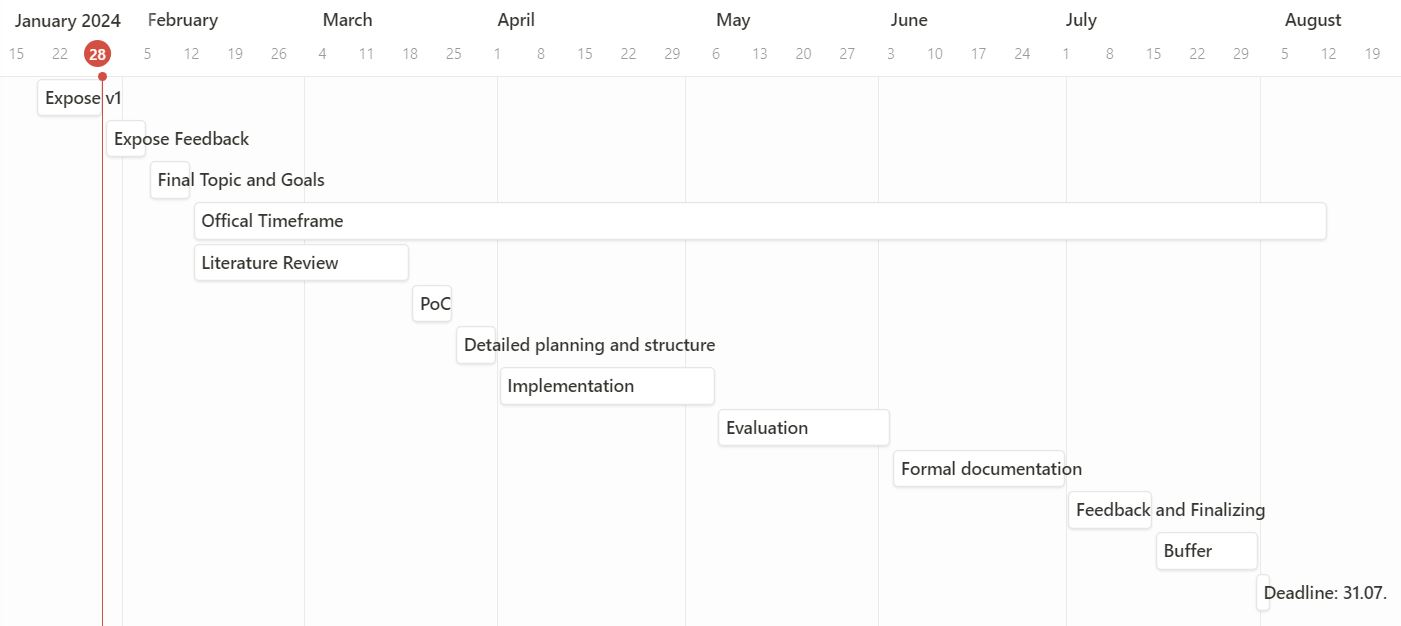
\includegraphics[width=1.2\textwidth]{images/timeline}}%
    \caption{Timeline}\label{fig:timeline}
\end{figure}%
